%!TEX root = ../main.tex

\chapter{Application of the Model}\label{cha:applying-model}

In this Chapter a method for assessing the sensitivity of the model will be outlined.
This is done by making small changes to the parameters of strategies and observing whether the model can discriminate between the original strategy and the altered version.
The size of the change made to the strategy will be varied and the models performance recorded for each deviation.
It is expected that there is a cut-off where the model changes from performing well to performing badly, and this gives an approximation of it's sensitivity.
Finally, model will be applied to the Axelrod-Python library to determine if it contains any duplicate strategies.



\section{MemoryOne Strategies}

A MemoryOne strategy bases its decision entirely on the the last round of play.
In Axelrod-Python they are defined by a vector $v$ of length 4 that determines the probability of Cooperation given the previous rounds history, ie:
$$
v = (P(C|CC), P(C|CD), P(C|DC), P(C|DD))
$$
For example, a MemoryOne strategy defined by the vector $v=(1, 1, 1, 1)$ is equivalent to Cooperator.
TitForTat can be implemented as a MemoryOne player with the vector $v=(1, 0, 1, 0)$, Pavlov as the MemoryOne player with $v=(1, 0, 0, 1)$ and Random as the MemoryOne player with $v=(0.5, 0.5, 0.5, 0.5)$.
See Section \ref{sec:individual_strategies} for explanations of how these strategies operate.



\section{Determining the sensitivity of the Model}




\section{Applying Model to Axelrod-Python}


\begin{figure}[htbp!]
    \centering
    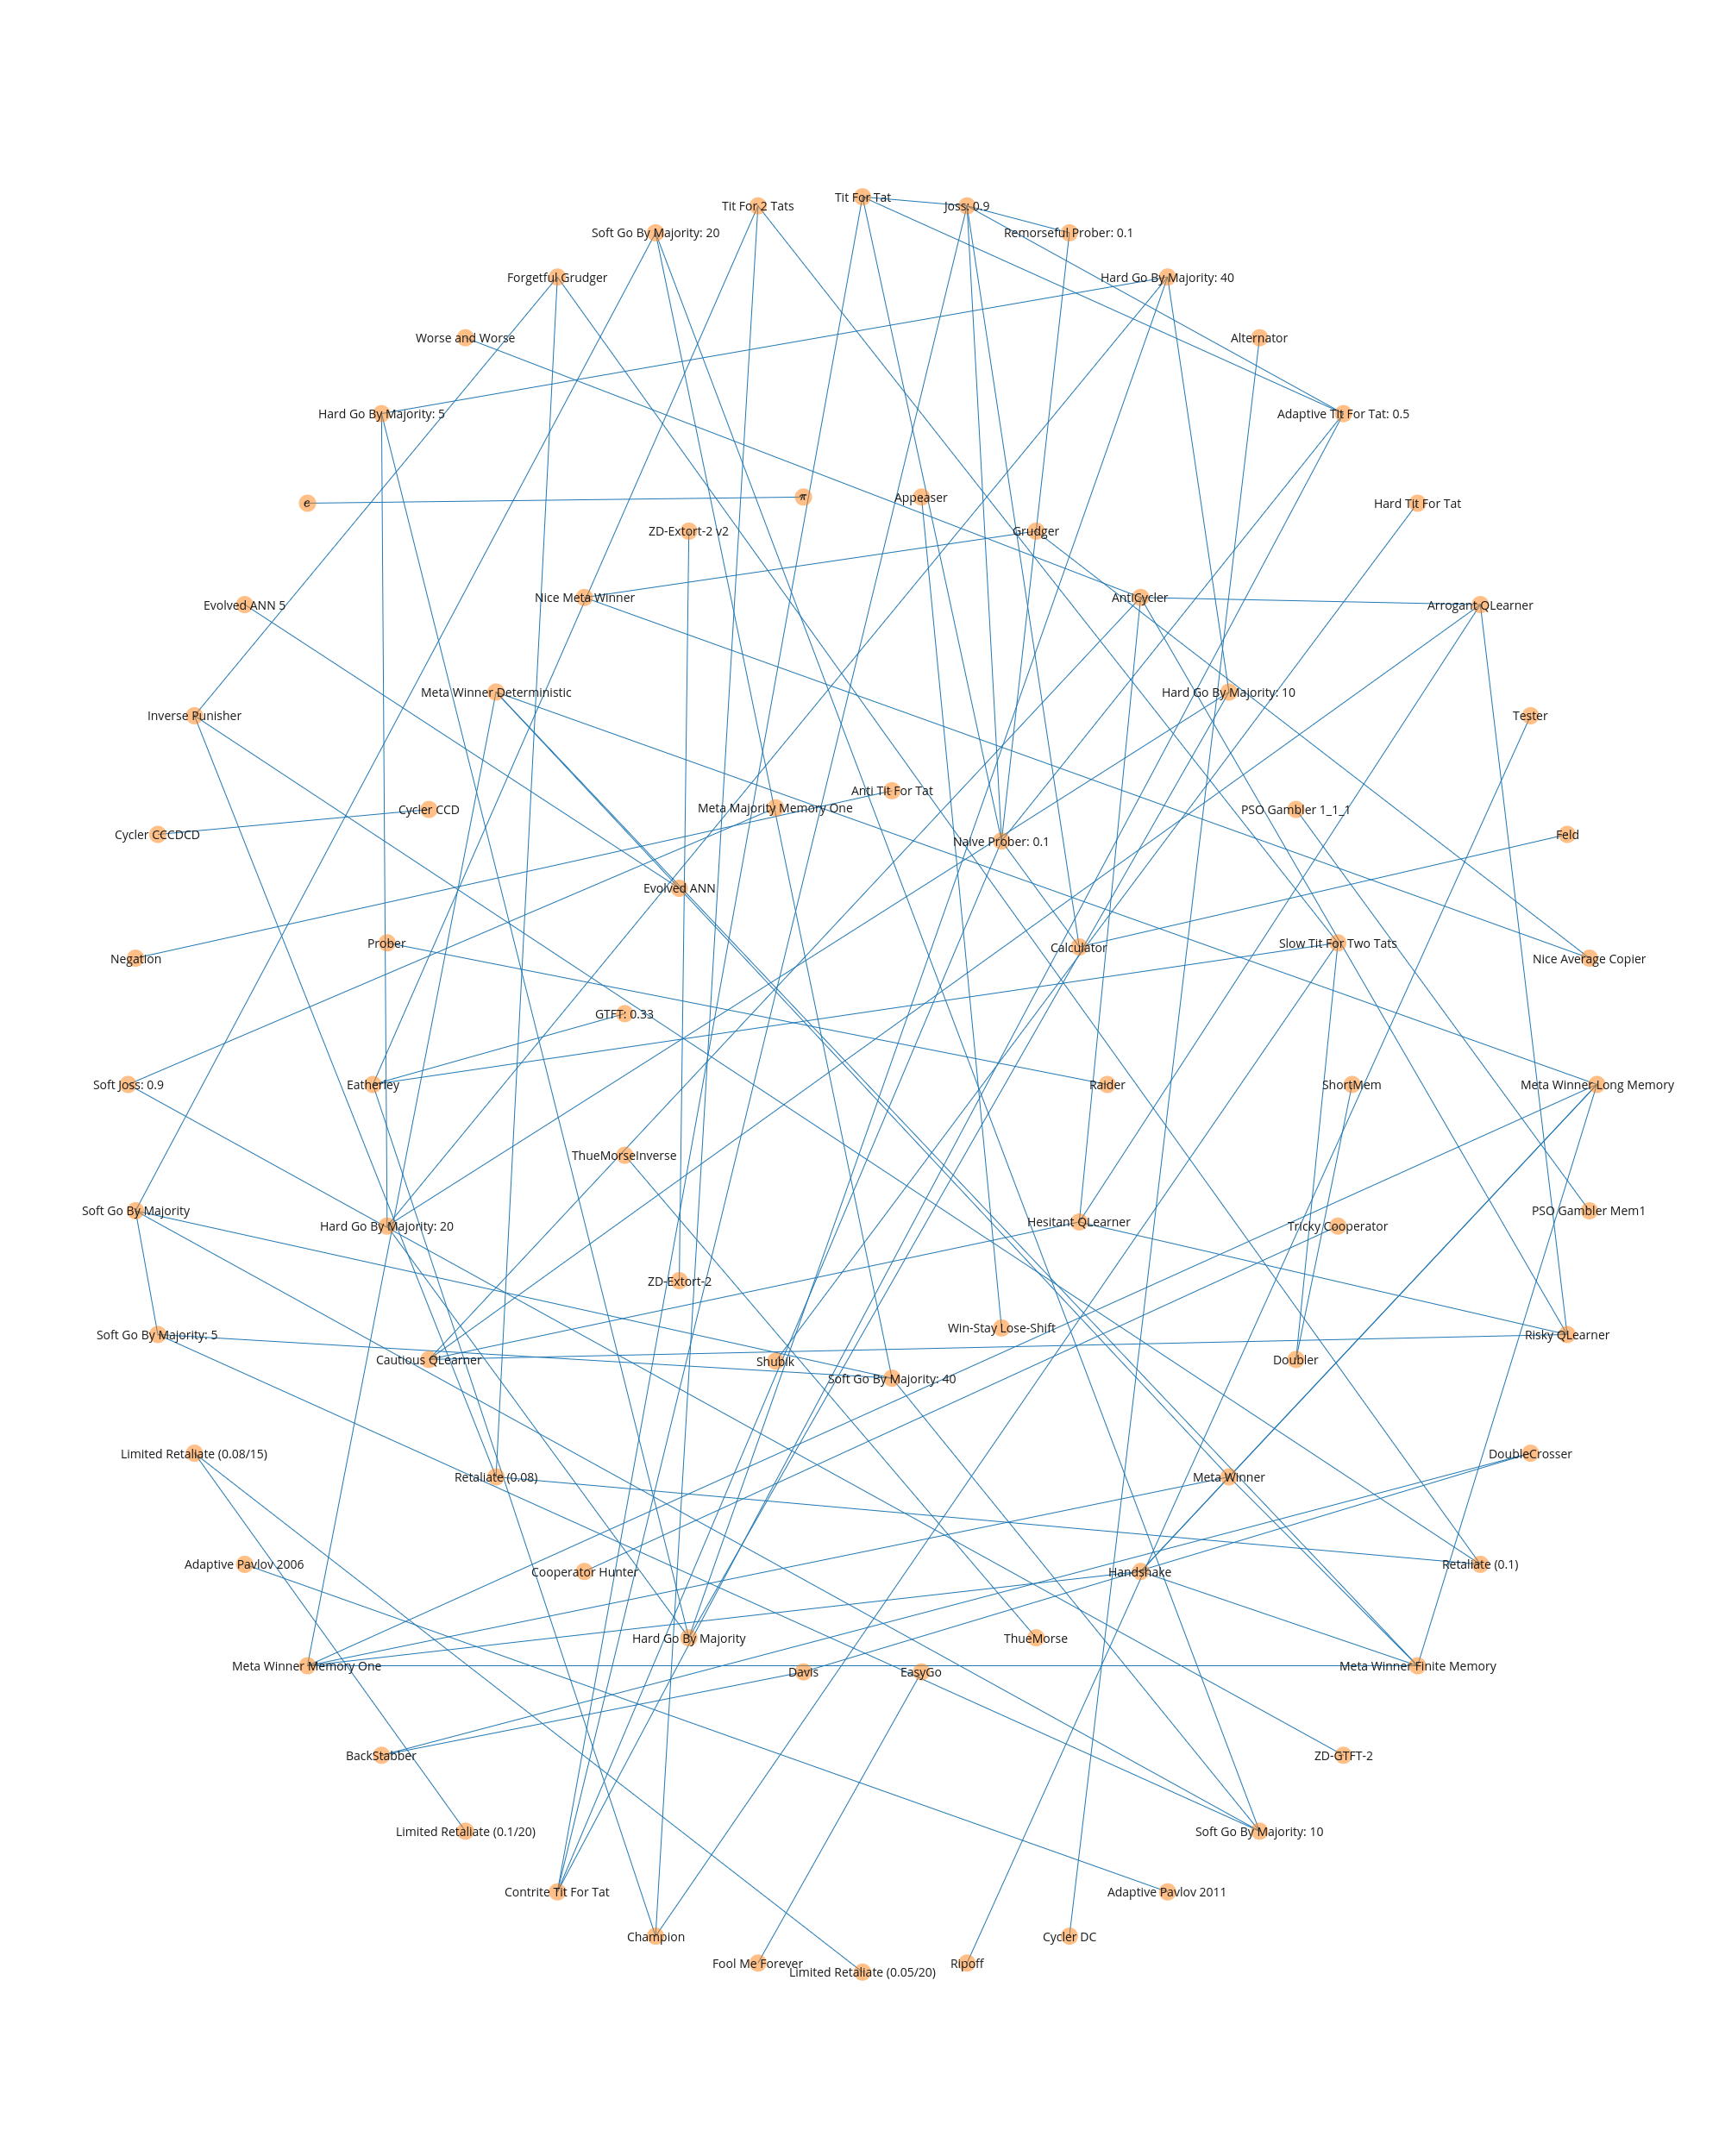
\includegraphics[width=\linewidth]{../img/neighbourhoods/overall.png}
    \caption{Caption here}
    \label{fig:figure1}
\end{figure}

\begin{figure}[htbp!]
\subfloat[]{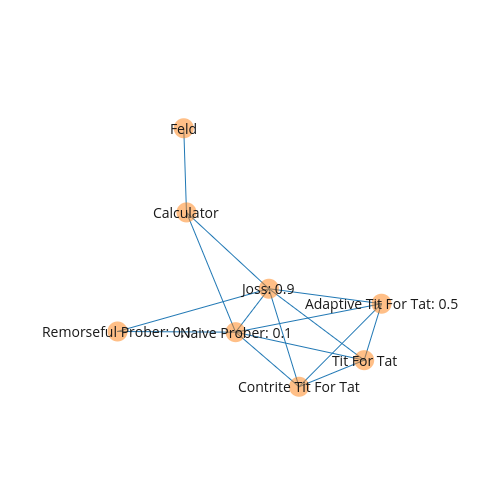
\includegraphics[width = 0.3\textwidth]{../img/neighbourhoods/1.png}}
\subfloat[]{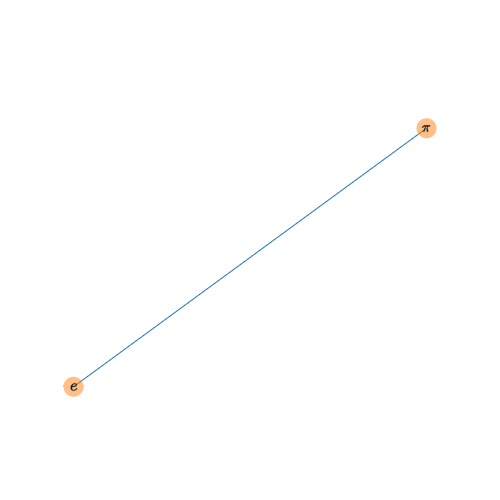
\includegraphics[width = 0.3\textwidth]{../img/neighbourhoods/10.png}}
\subfloat[]{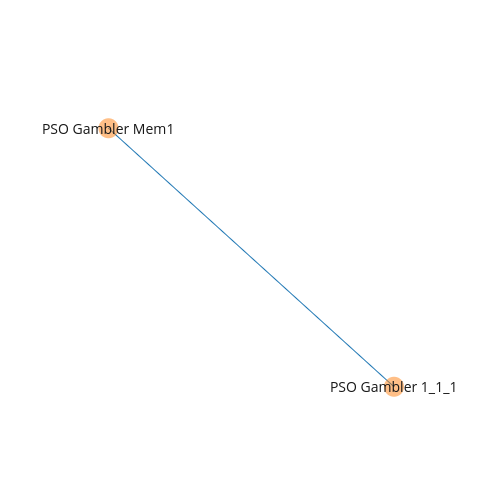
\includegraphics[width = 0.3\textwidth]{../img/neighbourhoods/102.png}} \\
\end{figure}
\begin{figure}[htbp!]
\ContinuedFloat
\subfloat[]{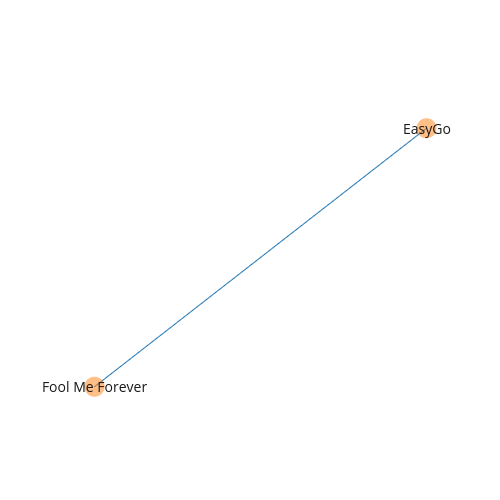
\includegraphics[width = 0.3\textwidth]{../img/neighbourhoods/107.png}}
\subfloat[]{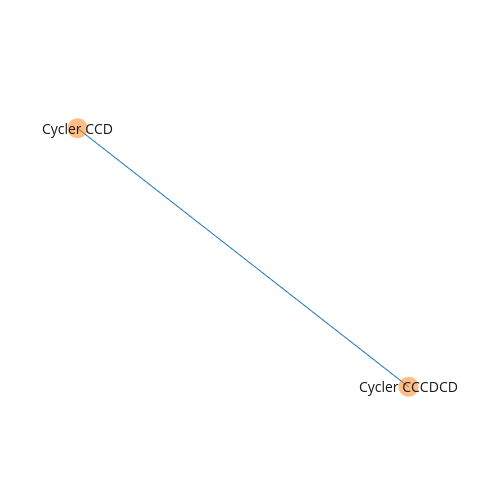
\includegraphics[width = 0.3\textwidth]{../img/neighbourhoods/12.png}}
\subfloat[]{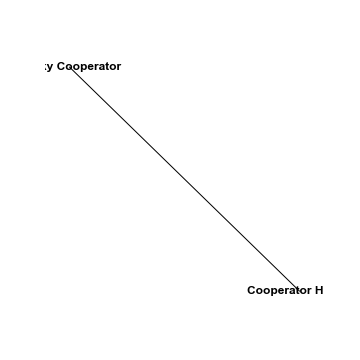
\includegraphics[width = 0.3\textwidth]{../img/neighbourhoods/16.png}} \\
\end{figure}
\begin{figure}[htbp!]
\ContinuedFloat
\subfloat[]{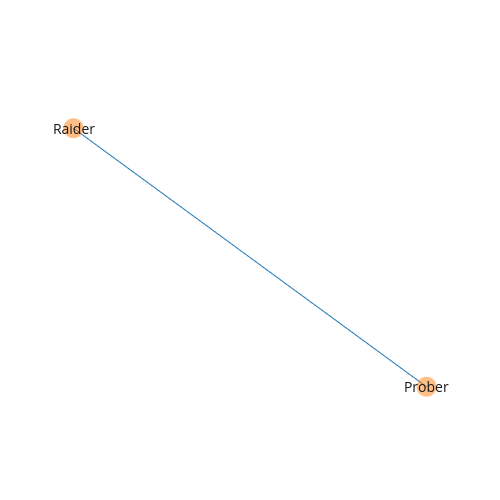
\includegraphics[width = 0.3\textwidth]{../img/neighbourhoods/17.png}}
\subfloat[]{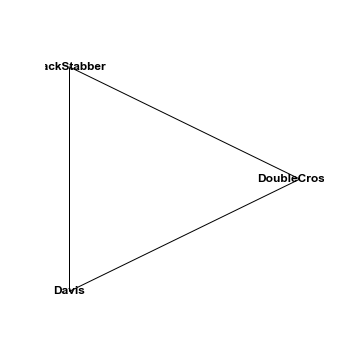
\includegraphics[width = 0.3\textwidth]{../img/neighbourhoods/18.png}}
\subfloat[]{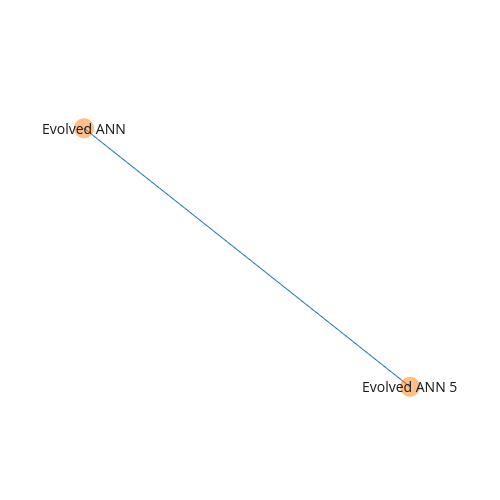
\includegraphics[width = 0.3\textwidth]{../img/neighbourhoods/2.png}} \\
\end{figure}
\begin{figure}[htbp!]
\ContinuedFloat
\subfloat[]{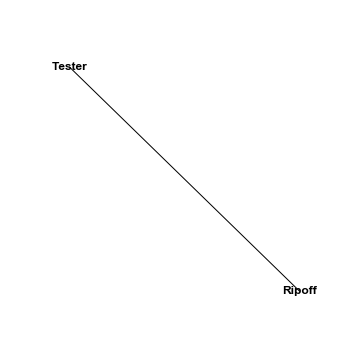
\includegraphics[width = 0.3\textwidth]{../img/neighbourhoods/22.png}}
\subfloat[]{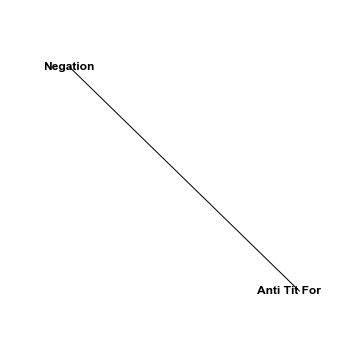
\includegraphics[width = 0.3\textwidth]{../img/neighbourhoods/24.png}}
\subfloat[]{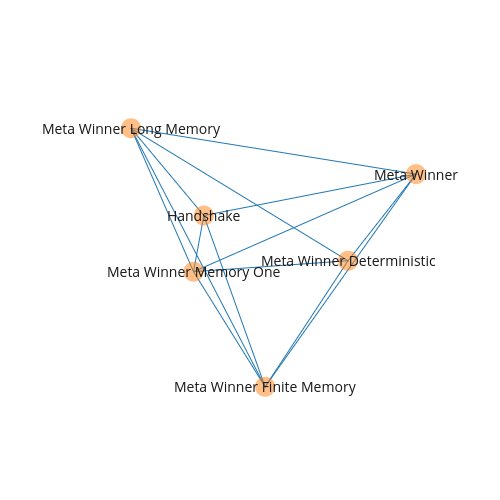
\includegraphics[width = 0.3\textwidth]{../img/neighbourhoods/29.png}} \\
\end{figure}
\begin{figure}[htbp!]
\ContinuedFloat
\subfloat[]{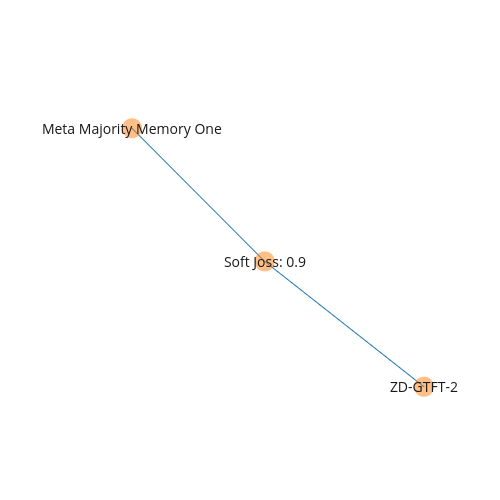
\includegraphics[width = 0.3\textwidth]{../img/neighbourhoods/30.png}}
\subfloat[]{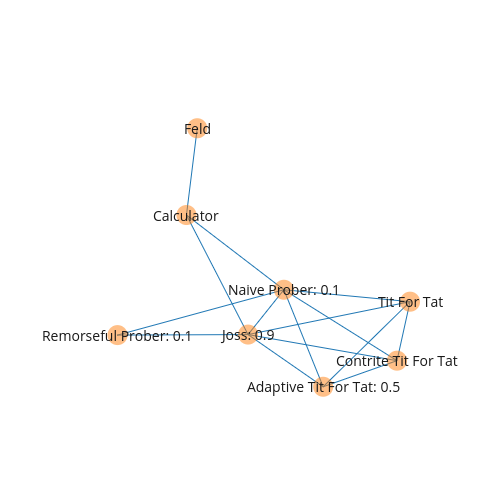
\includegraphics[width = 0.3\textwidth]{../img/neighbourhoods/31.png}}
\subfloat[]{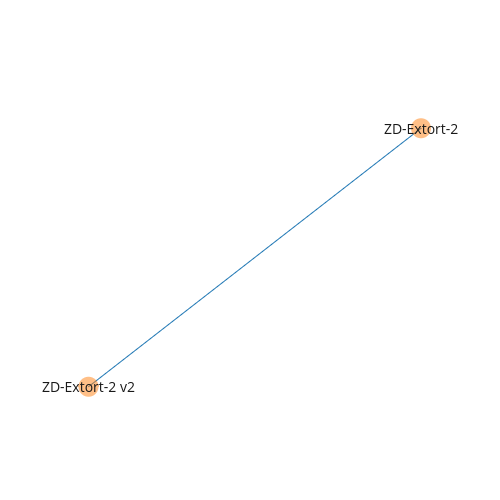
\includegraphics[width = 0.3\textwidth]{../img/neighbourhoods/36.png}} \\
\end{figure}
\begin{figure}[htbp!]
\ContinuedFloat
\subfloat[]{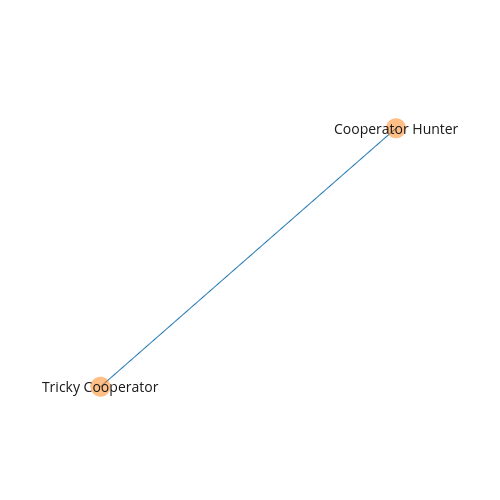
\includegraphics[width = 0.3\textwidth]{../img/neighbourhoods/38.png}}
\subfloat[]{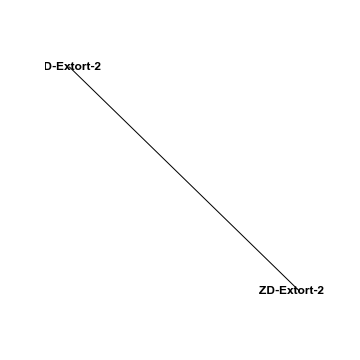
\includegraphics[width = 0.3\textwidth]{../img/neighbourhoods/4.png}}
\subfloat[]{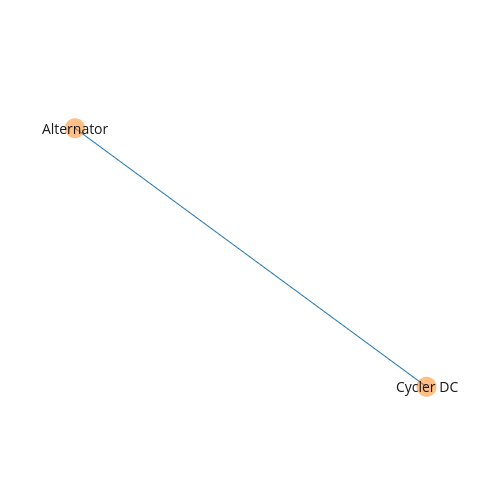
\includegraphics[width = 0.3\textwidth]{../img/neighbourhoods/47.png}} \\
\end{figure}
\begin{figure}[htbp!]
\ContinuedFloat
\subfloat[]{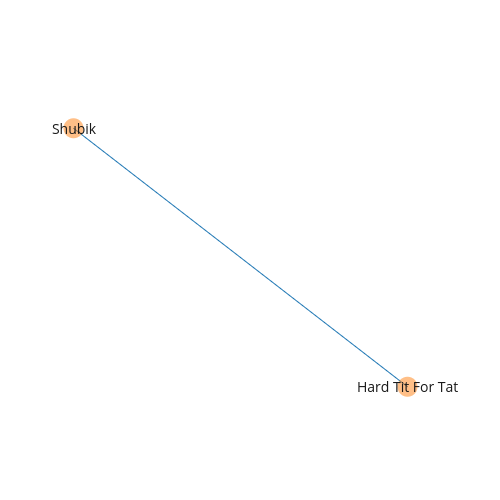
\includegraphics[width = 0.3\textwidth]{../img/neighbourhoods/49.png}}
\subfloat[]{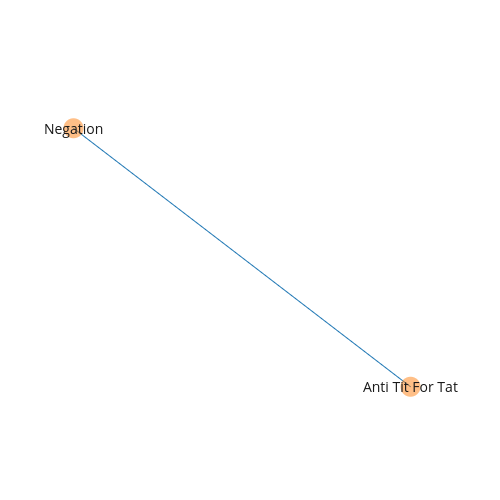
\includegraphics[width = 0.3\textwidth]{../img/neighbourhoods/55.png}}
\subfloat[]{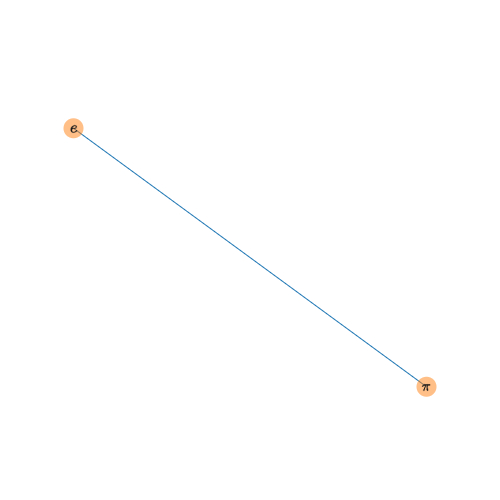
\includegraphics[width = 0.3\textwidth]{../img/neighbourhoods/58.png}} \\
\end{figure}
\begin{figure}[htbp!]
\ContinuedFloat
\subfloat[]{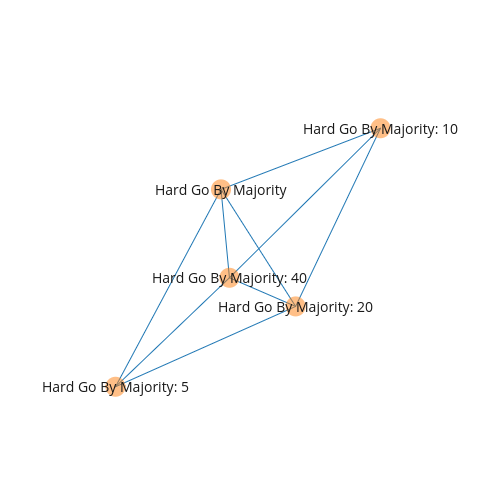
\includegraphics[width = 0.3\textwidth]{../img/neighbourhoods/60.png}}
\subfloat[]{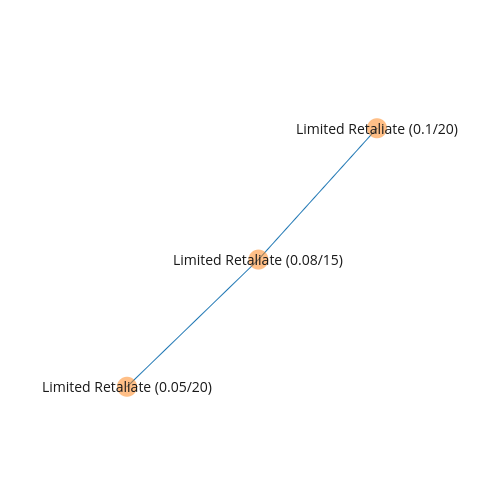
\includegraphics[width = 0.3\textwidth]{../img/neighbourhoods/7.png}}
\subfloat[]{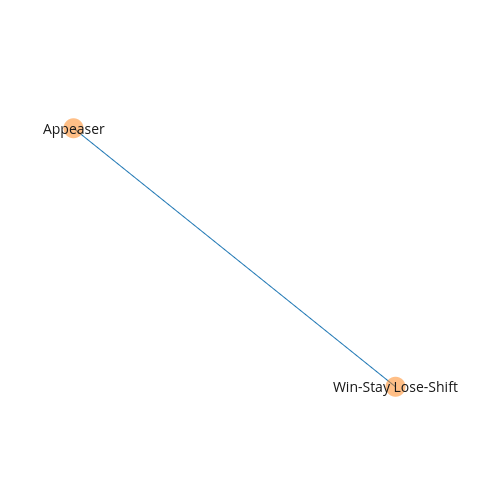
\includegraphics[width = 0.3\textwidth]{../img/neighbourhoods/74.png}} \\
\end{figure}
\begin{figure}[htbp!]
\ContinuedFloat
\subfloat[]{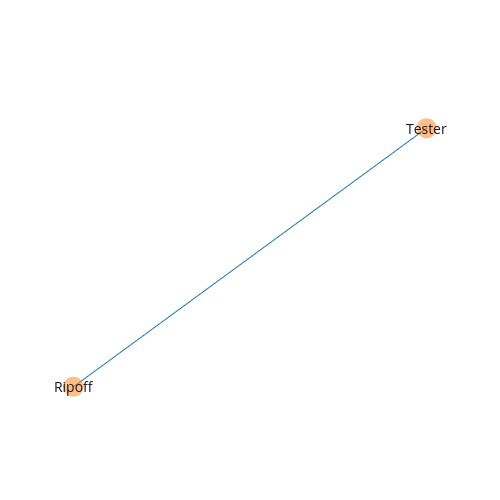
\includegraphics[width = 0.3\textwidth]{../img/neighbourhoods/78.png}}
\subfloat[]{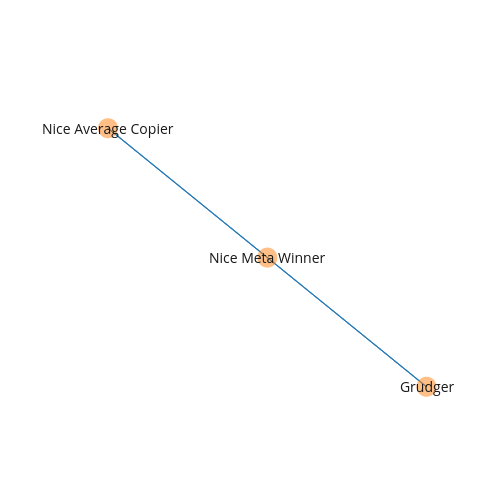
\includegraphics[width = 0.3\textwidth]{../img/neighbourhoods/84.png}}\\
\end{figure}
